\section{Systemmodel}
	\subsection{System structure}
			\subsubsection{Modules}
				INSERT SYSTEMMODELCHART HERE
				The main architecture pattern the system is oriented to, is the Model-View-Controller. But 				only the main structure, the architecture should be seen as parallel model.
			\subsubsection{Controller}
				The Controller is basically the whole scheduler-module. It controls the data flow with the 				data structure(Model) and the Data Mining-module which both of them are part of the 						scheduler. Furthermore, the scheduler is responsible for the communication with the code-             				and executer interface and the MPI-world. There will be a scientific code bound to the 						scheduler and executed with different tasks(different parameter input), those will be 						brought in order through the scheduler. This will be organized with special scheduler 						algorithms depend on the data mining and the statistics
			\subsubsection{Model}
				The Model is represented as an high performance file system. Data which will be collected 					for statistics will be stored in such a file in the file system. Also the data for 							bookkeeping with information about the progress of the tasks which are executed on the 						computer cluster will be stored in one file. The queue of the task order will be also 						placed in a file. 
			\subsubsection{View}
				The essential point of visualization will be the graphical output of the collected data. 					Bookkeeping and statistic can be plotted after the calculation.
				A GUI is a nice-to-have feature and is first of all not in planning. The input for the 						controller will be managed trough the MOAB Interface.

\subsection{Scenarios}
			szenario
\subsection{Use cases}
			need to be scaled
			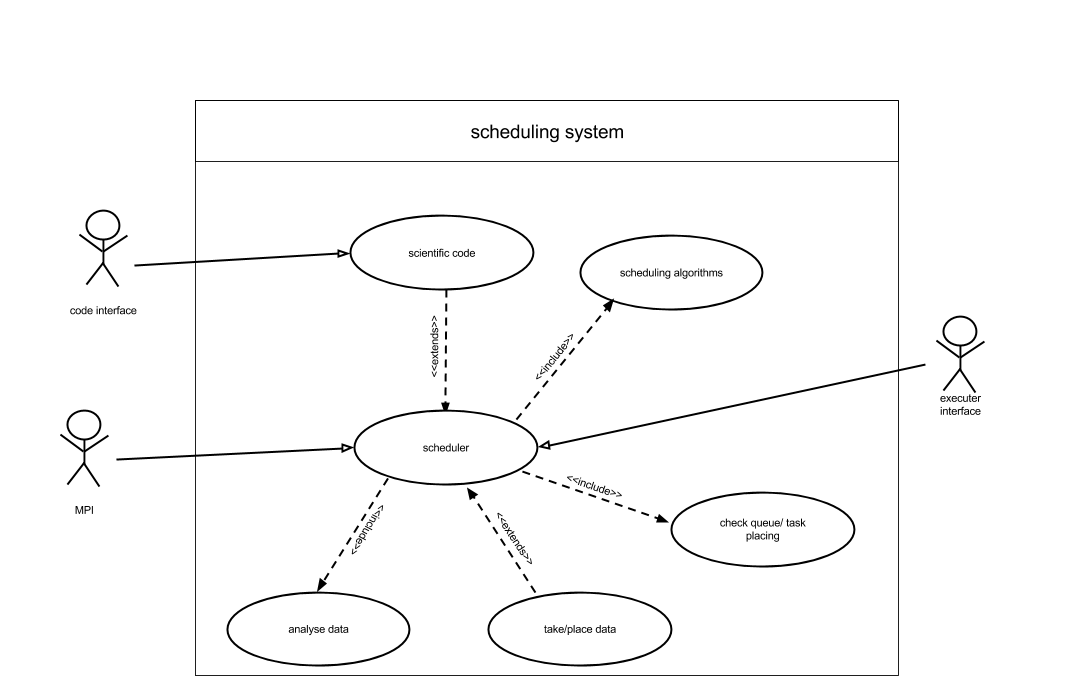
\includegraphics[width=1.4\textwidth]{usecasediagram.pdf}
			
\subsection{Object model}

\subsection{Dynamic models}

\subsection{Graphical user interface}
			maybe